% 第 22 题：打点计时器打出的纸带（A–E 五个计数点，位置按原图读数）
% 原图读数近似：A≈0.00、B≈1.00、C≈2.20、D≈4.20、E≈7.20 cm
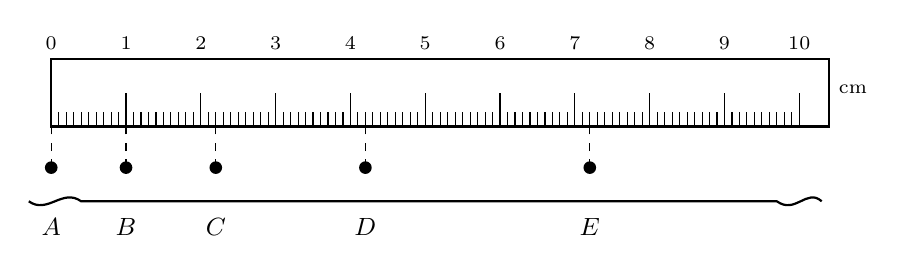
\begin{tikzpicture}[font=\small, scale=0.95]
  % 刻度尺
  \draw[thick] (0.2,1.6) rectangle (10.6,2.5);
  \foreach \i in {0,1,...,10} {
    \draw (0.2+\i,1.6) -- (0.2+\i,2.05);
    \node[above,font=\scriptsize] at (0.2+\i,2.5) {\i};
  }
  \foreach \i in {0,1,...,100} {
    \draw ({0.2+0.1*\i},1.6) -- ({0.2+0.1*\i},1.8);
  }
  \node[right,font=\scriptsize] at (10.6,2.1) {cm};
  % 纸带
  \draw[thick] (-0.1,0.6) .. controls (0.15,0.42) and (0.35,0.78) .. (0.6,0.6)
      -- (9.9,0.6) .. controls (10.15,0.42) and (10.3,0.78) .. (10.5,0.6);
  % 五个计数点（按原图读数定位）
  \foreach \x/\lab in {0.2/A,1.2/B,2.4/C,4.4/D,7.4/E} {
    \fill (\x,1.05) circle (2.4pt);
    \draw[dashed] (\x,1.05) -- (\x,1.6);
    \node[below] at (\x,0.5) {$\lab$};
  }
\end{tikzpicture}
